\documentclass[12pt]{report}

\usepackage{graphicx}
\usepackage{float}
\usepackage{biblatex}
\usepackage[a4paper, margin=1in]{geometry}

\makeatletter
\renewcommand{\maketitle}{
\begin{center}

\pagestyle{empty}
\phantom{.}  %necessary to add space on top before the title
\vspace{0.5cm}

{\Huge \bf \@title\par}
\vspace{5cm}

{\LARGE Zülal Uludoğan, }\\[0.5cm]
{\LARGE Ahmet Taha Çelik, 2515831}

\vfill

{\Large\@date}

\end{center}
}\makeatother

\title{EE446 Term Project Report \\ Middle East Technical University}
\author{Ahmet Taha Çelik, Zülal Uludoğan}
\date{25 May 2025}

\begin{document}

\maketitle
\tableofcontents

\chapter{Introduction}

\section{Project Description}


\chapter{Datapath Module}


\chapter{Controller Module}

\paragraph{}
The controller module is responsible for generating the control signals necessary to guide the datapath during the execution of RISC-V instructions. As shown in Figure \ref{fig:controller}, the controller design follows a modular approach and includes three functional units: the \texttt{MainDecoder}, the \texttt{ALUDecoder}, and the \texttt{PCLogic} unit.

\begin{figure}[h]
    \centering
    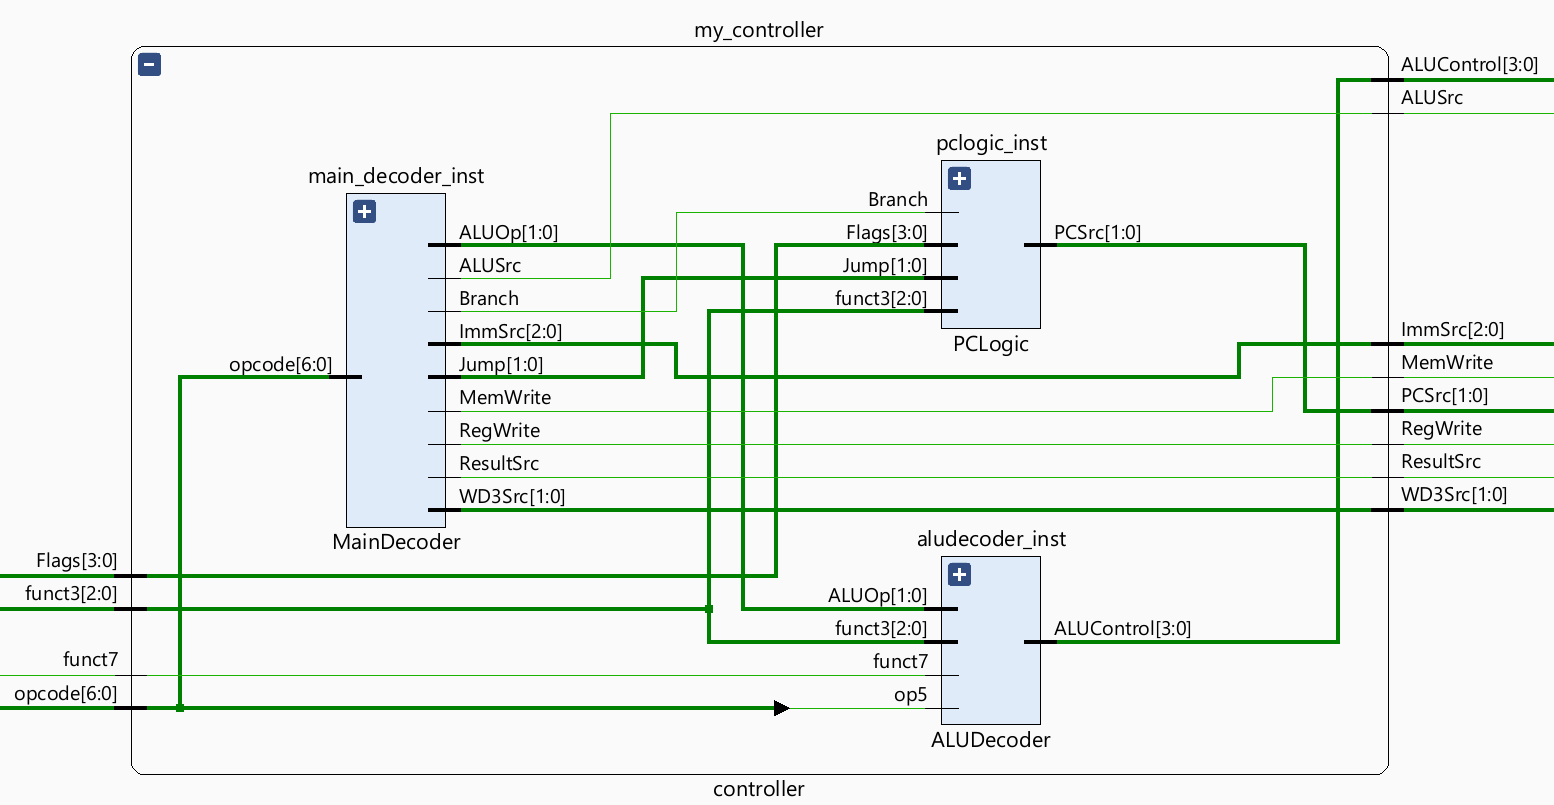
\includegraphics[width=\textwidth]{figures/controller_rtl.png}
    \caption{Synthesized RTL view of the controller module}
    \label{fig:controller}
\end{figure}

\paragraph{}
The \texttt{MainDecoder} interprets the 7-bit opcode from the instruction and produces the primary control signals required by the datapath, such as register file write enable, memory write enable, ALU source selection, and immediate format selection. These signals are then distributed to the corresponding components to orchestrate the processor's behavior.

\paragraph{}
The \texttt{ALUDecoder} further refines control signal generation by examining the \texttt{funct3}, \texttt{funct7}, and other opcode-specific bits to determine the specific ALU operation to perform. It outputs a 4-bit \texttt{ALUControl} signal, ensuring the correct arithmetic or logical operation is selected based on the instruction type.

\paragraph{}
The \texttt{PCLogic} unit handles program counter selection. It considers both the branching conditions and the jump instructions to compute the correct value of the \texttt{PCSrc} signal. This logic is critical for implementing both conditional and unconditional control-flow changes in the processor.

\paragraph{}
The modularity of this controller design simplifies debugging and testing. Each submodule is implemented independently and tested in isolation before integration into the main controller unit.


\chapter{UART Module}

\paragraph{}
The UART (Universal Asynchronous Receiver-Transmitter) module is responsible for facilitating serial communication between the RISC-V processor and external systems. Its implementation involved significantly more complexity than the controller module due to the nature of asynchronous communication, timing constraints, and the need to bridge two separate clock domains. Figure \ref{fig:uart} shows the synthesized RTL view of the UART subsystem.

\begin{figure}[h]
    \centering
    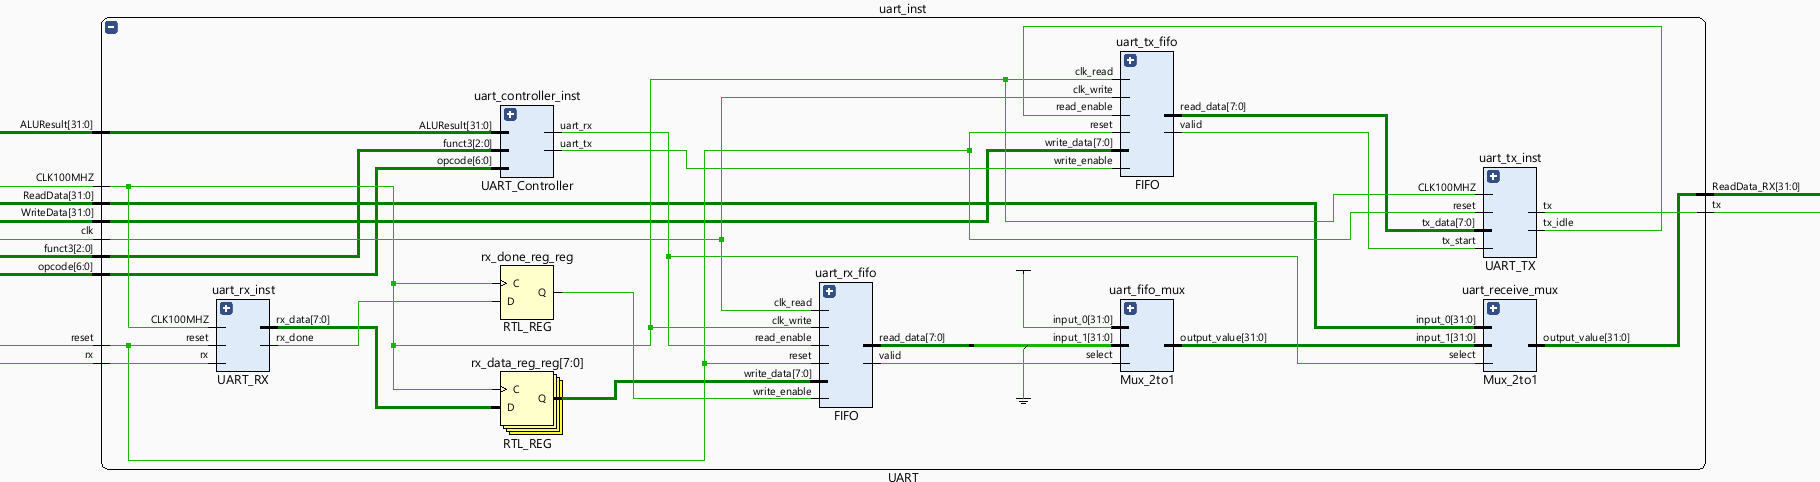
\includegraphics[width=\textwidth]{figures/uart_rtl.png}
    \caption{Synthesized RTL view of the UART module}
    \label{fig:uart}
\end{figure}

\section*{Design Overview}

\paragraph{}
The UART module integrates both transmitting and receiving functionalities while adhering to the 9600 baud 8-N-1 protocol. Memory-mapped I/O is used to send and receive bytes via store and load instructions to addresses \texttt{0x400} and \texttt{0x404}, respectively. When a store is made to \texttt{0x400}, a byte is written to the transmitter FIFO and scheduled for transmission. When a load is performed from \texttt{0x404}, the system reads the most recent byte from the receive FIFO; if no byte is available, the value \texttt{0xFFFFFFFF} is returned.

\paragraph{}
The UART controller examines the current instruction's opcode, \texttt{funct3}, and ALU result to determine whether a UART send or receive should be triggered. This controller outputs \texttt{uart\_tx} or \texttt{uart\_rx} flags accordingly.

\section{Clock Domain Challenges and FIFO Synchronization}

\paragraph{}
One of the key challenges in designing the UART module was handling the presence of two independent clocks: a 100 MHz clock (\texttt{CLK100MHZ}) required for UART transmission timing, and a manually generated system clock (\texttt{clk}) used by the rest of the processor, including the register file and instruction control. Since UART must transmit data at precise intervals defined by the baud rate, it must operate continuously using \texttt{CLK100MHZ}. However, if both the UART and the register file accessed the same FIFO at their own clock rates without isolation, it would introduce race conditions and data corruption.

\paragraph{}
To address this, the design includes dual-clock FIFOs that are explicitly controlled with separate clock signals: \texttt{clk\_write} and \texttt{clk\_read}. The write side of the FIFO operates on \texttt{CLK100MHZ}, synchronized with \texttt{UART\_RX} and \texttt{UART\_TX} modules, while the read side operates on the processor’s \texttt{clk}, ensuring that data transfer from UART into the register file occurs safely. This separation of clock domains is essential to maintain system stability and correctness across asynchronous boundaries.

\section{UART Transmitter and Receiver}

\paragraph{}
The transmitter module initiates data transmission when a byte is enqueued into the FIFO and the line is idle. It serializes the data byte according to UART protocol and asserts the \texttt{tx\_idle} signal once transmission is complete. If the FIFO holds multiple bytes, they are transmitted sequentially without processor intervention.

\paragraph{}
The receiver module continuously samples the input \texttt{rx} line using \texttt{CLK100MHZ}. When a valid start bit is detected, it begins capturing bits until the full byte is received. A \texttt{done} flag is raised once reception is complete. The received byte is then pushed into the 16-byte FIFO buffer, ensuring that no bytes are lost if the processor is not immediately ready to read.

\section*{UART Transmitter and Receiver State Machines}

\paragraph{}
Both the UART transmitter and receiver modules are implemented as finite state machines (FSMs) that operate on the 100 MHz clock and comply with the 9600 baud 8-N-1 UART protocol. Their behaviors are structured as sequential state transitions, and the FSM logic ensures the correct serialization and deserialization of data.

\subsection*{Transmitter State Machine}

\paragraph{}
The transmitter FSM begins in the \texttt{IDLE} state, where it waits for the \texttt{start} signal to be asserted, indicating that a new byte is ready for transmission. Upon activation, it transitions to the \texttt{START} state and drives the transmission line low to indicate the start bit. After holding the line low for one baud period, the FSM enters the \texttt{DATA} state, during which each of the 8 data bits is shifted out sequentially, least significant bit first.

\paragraph{}
Once all data bits are transmitted, the FSM transitions to the \texttt{STOP} state. It then drives the line high for one baud period to signal the stop bit. After this, the FSM returns to the \texttt{IDLE} state, sets the \texttt{idle} flag to indicate readiness, and awaits the next start signal.

\paragraph{}
This structure ensures that every byte is framed with a start and stop bit as per UART standards, and the \texttt{idle} output allows external logic to determine when the transmitter is available for the next byte.

\subsection{Receiver State Machine}

\paragraph{}
The receiver FSM also begins in an \texttt{IDLE} state, continuously monitoring the input \texttt{rx} line. Upon detecting a falling edge (start bit), it transitions to the \texttt{START} state and waits half a baud period to sample the start bit in the middle for noise immunity.

\paragraph{}
After verifying the start bit, it transitions to the \texttt{DATA} state, where it samples 8 data bits at one baud interval each. These bits are shifted into a register, with the least significant bit arriving first.

\paragraph{}
Following the data bits, the FSM enters the \texttt{STOP} state to sample the stop bit. If the stop bit is valid (logic high), the FSM sets the \texttt{done} flag and updates the \texttt{data\_out} register with the fully received byte. It then returns to the \texttt{IDLE} state to prepare for the next frame.

\paragraph{}
This approach ensures that bytes are received reliably and with proper framing. The \texttt{done} signal is used to indicate reception completion, allowing external logic to push the received byte into a FIFO buffer or register.

\section{Peripheral Interface and Muxing}

\paragraph{}
The UART module includes additional logic for interfacing with the processor. When a load operation targets the UART receive address, a multiplexer determines whether valid data exists in the FIFO. If not, it returns \texttt{0xFFFFFFFF}, as required by the design specification. Similarly, when a store operation targets the transmit address, a different multiplexer ensures that the byte written by the processor is passed correctly to the transmit FIFO, provided the transmitter is not currently busy.

\paragraph{}
With careful clock domain handling, FIFO synchronization, and protocol adherence, the UART module operates as a robust peripheral enabling reliable serial communication within the single-cycle RISC-V system.

\chapter{Cocotb Testbench}


\end{document}